%-------------------------------To - Do List-------------------------------------------------
%1.  For section 3.2 for LocMetrics, need a talk a little more about it and
%		add the graphs.
%2. For section 4 we need to talk a little more about Understand C++
%		as our primary extraction tool
%3. Section 8 control flow. I didnt know what to do here
%4. Section 9 Should we add the diagram for the header files here? Where
%		would that ideally go
%5. Section 11 conclusion needs to be added
%6. Should we add an abstract?
%7. Citations need to be updated/added
%8. (Bryan) I can print the document and get a simple folder from dollarama
% 	to add it to but lets finish this by tonight or tomorrow morning so 
%		we don't need to spend too much time on it.
%-----------------------------------------------------------------------------------------------
%%%%%%%%%%%%%%%%%%%%%%%%%%%%%%%%%%%%%%%%%
% University Assignment Title Page 
% LaTeX Template
% Version 1.0 (27/12/12)
%
% This template has been downloaded from:
% http://www.LaTeXTemplates.com
%
% Original author:
% WikiBooks (http://en.wikibooks.org/wiki/LaTeX/Title_Creation)
%
% License:
% CC BY-NC-SA 3.0 (http://creativecommons.org/licenses/by-nc-sa/3.0/)
% 
% Instructions for using this template:
% This title page is capable of being compiled as is. This is not useful for 
% including it in another document. To do this, you have two options: 
%
% 1) Copy/paste everything between \begin{document} and \end{document} 
% starting at \begin{titlepage} and paste this into another LaTeX file where you 
% want your title page.
% OR
% 2) Remove everything outside the \begin{titlepage} and \end{titlepage} and 
% move this file to the same directory as the LaTeX file you wish to add it to. 
% Then add \input{./title_page_1.tex} to your LaTeX file where you want your
% title page.
%
%%%%%%%%%%%%%%%%%%%%%%%%%%%%%%%%%%%%%%%%%
%\title{Title page with logo}
%----------------------------------------------------------------------------------------
%   PACKAGES AND OTHER DOCUMENT CONFIGURATIONS
%----------------------------------------------------------------------------------------

\documentclass[12pt]{article}
\usepackage[english]{babel}
\usepackage[utf8x]{inputenc}
\usepackage{amsmath}
\usepackage{graphicx}
\usepackage[colorinlistoftodos]{todonotes}
\usepackage[document]{ragged2e}


\begin{document}

\begin{titlepage}

\newcommand{\HRule}{\rule{\linewidth}{0.5mm}} % Defines a new command for the horizontal lines, change thickness here

\center % Center everything on the page
 
%----------------------------------------------------------------------------------------
%   HEADING SECTIONS
%----------------------------------------------------------------------------------------

\textsc{\LARGE Dalhousie University}\\[1.5cm] % Name of your university/college
\textsc{\Large Topics in Program Comprehension}\\[0.5cm] % Major heading such as course name
\textsc{\large CSCI 6306}\\[0.5cm] % Minor heading such as course title

%----------------------------------------------------------------------------------------
%   TITLE SECTION
%----------------------------------------------------------------------------------------

\HRule \\[0.4cm]
{ \huge \bfseries Architecture Extraction}\\[0.4cm] % Title of your document
\HRule \\[1.5cm]
 
%----------------------------------------------------------------------------------------
%   AUTHOR SECTION
%----------------------------------------------------------------------------------------

~
%\begin{minipage}{0.4\textwidth}
%\begin{flushright} \large
\emph{Group : Something} \\
Bhupendra \textsc{Rajawat} \\
Bryan Thomas \textsc{D'silva}\\ % Supervisor's Name 
Saurabh \textsc{Singh}\\
\bigskip
%\end{flushright}
%\end{minipage}\\[2cm]

% If you don't want a supervisor, uncomment the two lines below and remove the section above
%\Large \emph{Author:}\\
%John \textsc{Smith}\\[3cm] % Your name

%----------------------------------------------------------------------------------------
%   DATE SECTION
%----------------------------------------------------------------------------------------

{\large \today}\\[2cm] % Date, change the \today to a set date if you want to be precise

%----------------------------------------------------------------------------------------
%   LOGO SECTION
%----------------------------------------------------------------------------------------


\includegraphics[width=0.7\textwidth]{dal.jpg}% Include a department/university logo - this will require the graphicx package
 
%----------------------------------------------------------------------------------------

\vfill % Fill the rest of the page with whitespace

\end{titlepage}
\newpage
\textbf{Note: Our fourth group member, Anto Anthony Arulappan had an emergency in the family and had to leave to India for the same. He has dropped the course and hence will no longer be a part of our group.}
\newpage
\tableofcontents
\newpage
\justify
\begin{abstract}
Like we already discussed in different presentation and even in class that to figure out the architecture of any application program comprehension is required.To do program comprehension either code must be properly written to give over all understanding or application documentation need to be done well to make other people understanding code a edge to grasp the logic easily. We went across different application which we have stated in next section and found Gimp to be most suitable in terms of code and documentation. Fulfilling the main aim of this assignment to get the better insight how to figure out high -level architecture we did used a mix approach of top-down and bottom-up approach along with taking help from well written documentation of Gimp present at http://wiki.gimp.org . 
\end{abstract}

\section{Finding a Software System}
We looked at the following software systems and games.
\begin{enumerate}
\item \textbf{Kodi}: Kodi is an open source software media player and entertainment hub. This is available on atleast seven platforms. This was one of the first softwares we looked at and kept it as a contender

\item \textbf{Quake III}: The source code for Quake is challenging and interesting. However, there is almost no documentation for the same and hence we decided not to go ahead with this for now.

\item \textbf{GIMP}: GIMP is a cross platform image editor with an excellent community backing it up. We decided to extract the architecture for GIMP. We talk more about GIMP in the further sections.

\end{enumerate}

We also looked at Doom3, SuperTuxKart, Wordpress, TuxRunner and Linux but found GIMP to be the most interesting one to use for this assignment
\section{About GIMP}
GIMP was designed initially as a General image manipulation program. This was later changed to GNU Image Manipulation Program. It is free and openly available to retouch and edit images, convert image formats and more specialized tasks targeted towards image manipulation. GIMP provides an interface to handle simple graphics needs without learning advanced methods for image manipulation. GIMP is more user friendly as compared to other photoshop techniques and can be modified to fit your needs. And the best part about it is that it is free.
\section{Tools}
\subsection{Count Lines of Code}
Count Lines of Code\cite{cloc}, abbreviated as CLOC is a software used to count comment lines, blank lines and physical lines of code. We used this software initially when we looked at what software system we need to pick. We can look at figure \ref{fig:clocgimp output for GIMP}  for the output for GIMP. To sum it we have 3,695,059 LOC. However, we would assume that the chunk of our work would be for C which sums to about 608,029 LOC.  
\begin{figure}[h]
	\centering
	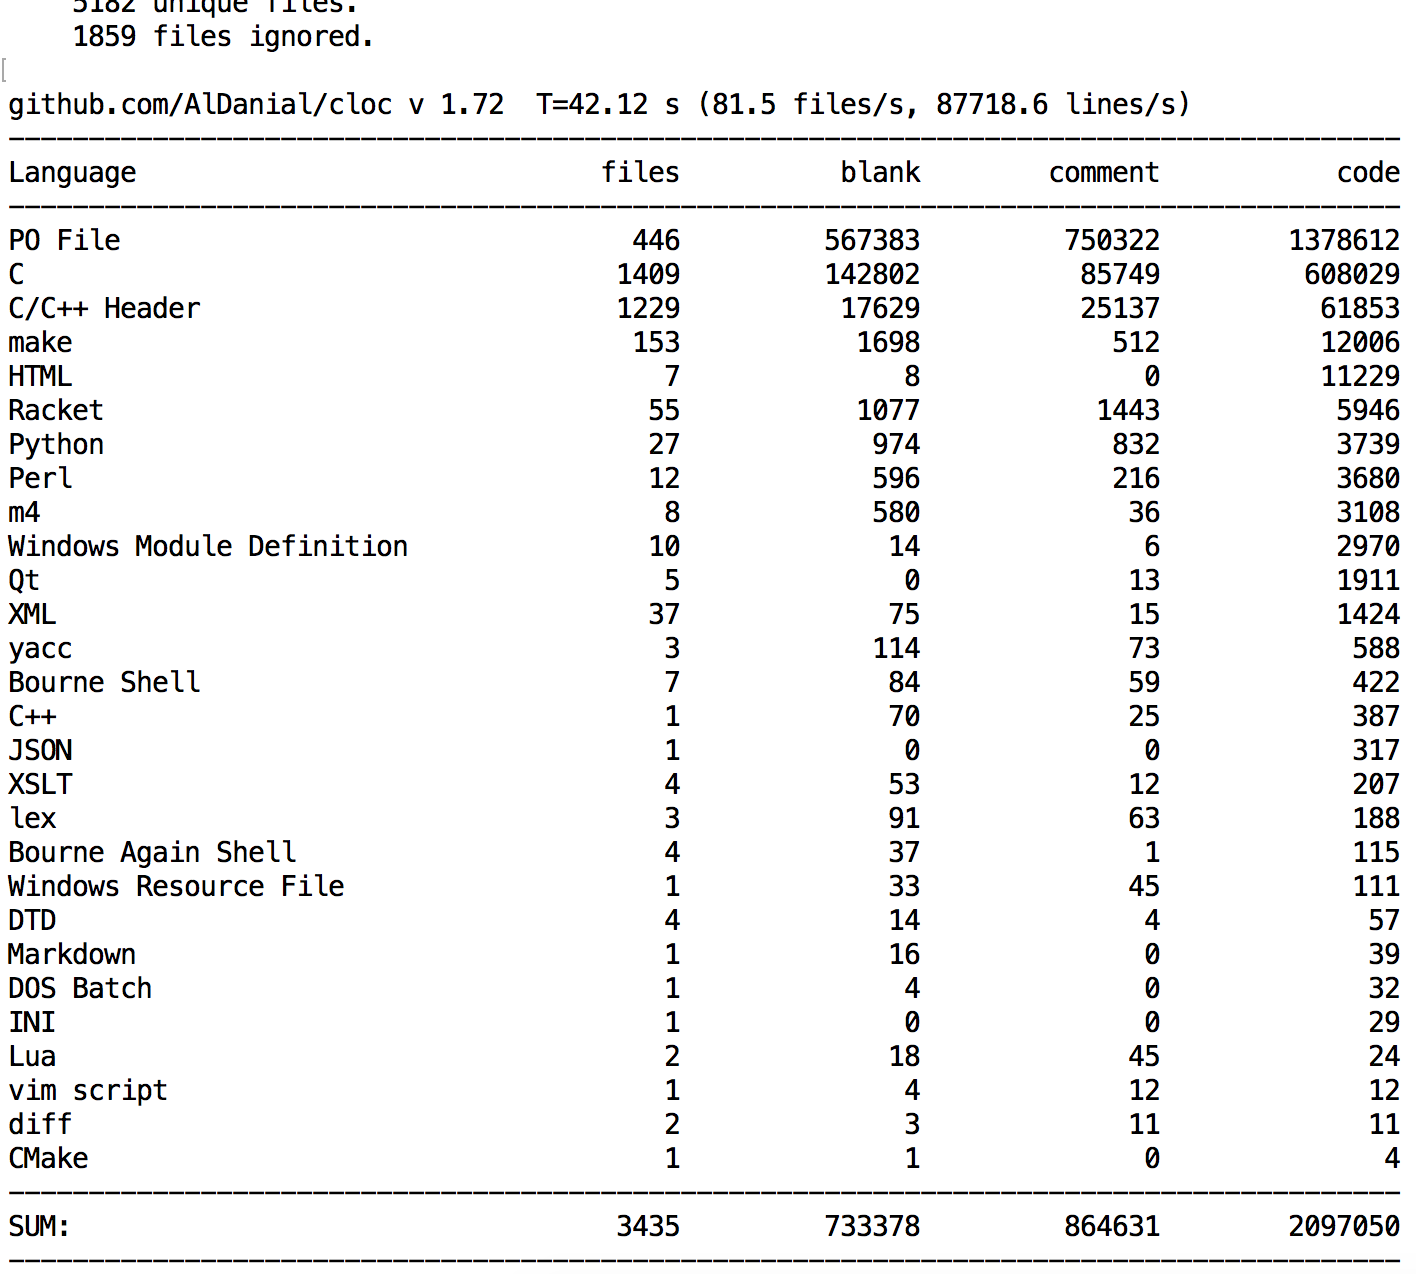
\includegraphics[width=0.7\linewidth, height=0.4\textheight]{clocgimp}
	\caption{clocgimp output for GIMP}
	\label{fig:clocgimp output for GIMP}
\end{figure}

%LocMetrics
\subsection{LocMetrics}
LocMetrics\cite{LocMetrics} is very similar to what CLOC does. We did find this software interesting because of how it visualized the output.LocMetrics counts total lines of code (LOC), blank lines of code (BLOC), comment lines of code, lines with both code and comments (C\&SLOC), logical source lines of code (SLOC-L), McCabe VG complexity (MVG), and number of comment words (CWORDS). Physical executable source lines of code (SLOC-P) is calculated as the total lines of source code minus blank lines and comment lines. Counts are calculated on a per file basis and accumulated for the entire project. LocMetrics also generates a comment word histogram. \cite{LocMetrics} 
\newline LocMetric has a very unique way to represent data which can be visualize in the figure \ref{fig:LocMetrics representaion of GIMP}
\begin{figure}[h]
	\centering
	\includegraphics[width=0.9\linewidth, height=0.5\textheight]{"Lines of code"}
	\caption{LocMetrics representaion of GIMP}
	\label{fig:LocMetrics representaion of GIMP}
\end{figure}
\subsection{Eclipse:}
For the analysis part of this application IDE used is Eclipse as it provide features that are interesting for C/C++ developers like Some of the features that are interesting for C/C++ developers are:
\textbf{cross-referencing:} Ctrl click an identifier and it will take you to its definition,
call hierarchy,
comprehensive search capabilities,
built in Git support,
Autotools integration,
graphical debugger,
explore remote systems from within Eclipse,
focus on the current task,
Bugzilla integration,
static code analysis.
and more. Eclipse runs on every platform that can run Java and has a graphical interface. Because of the above features Eclipse is good to use with the dependencies required for GIMP.
\section{Directory Structure}
We generated a butterfly diagram in figure \ref{fig:direc} for the directory structure. Using this and the documentation we did want to identify the main folder we would want to have a look at. We concluded that the app directory is the main directory that we are concerned about. It contains the source code for GIMP without any external tools or plugins. We would ideally ignore the modules, plugins and libraries for now and focus on the app directory. 
\begin{figure}[h]
\centering
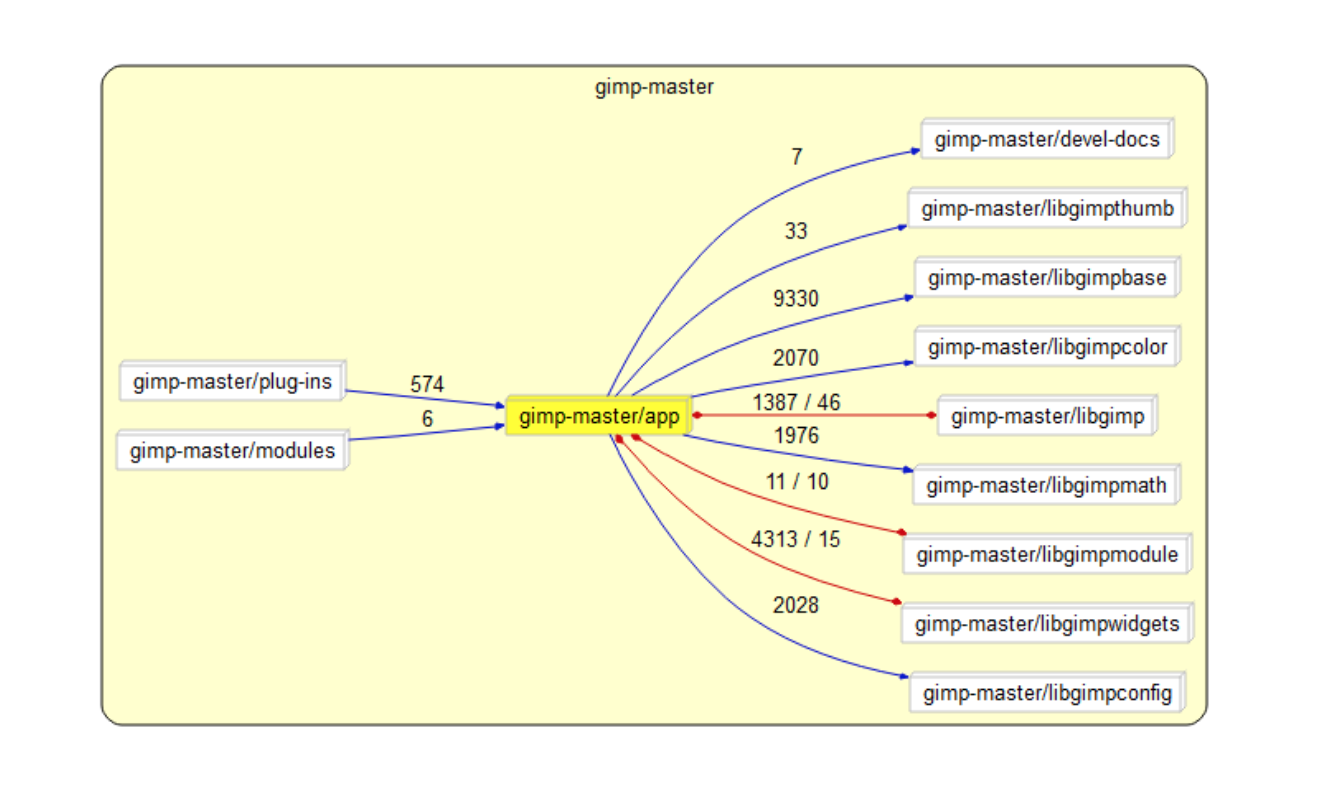
\includegraphics[width=1\textwidth]{directorybutterfly.png}
\caption{\label{fig:direc}Directory Structure}
\end{figure}
So we did the same for the app folder in figure \ref{fig:appfolder}. It was easy to comprehend since GIMP is very well organized with a good community support and documentation. The app/core directory is the guts of the GIMP software. Looking at the documentation provided for GIMP, major changes that need to be made start here. With the goal of refactoring in mind, this is where we would start, keeping in mind that changing files here will have an avalanche effect, so we need to be prepared for big changes in other files depending on these.
\begin{figure}
\centering
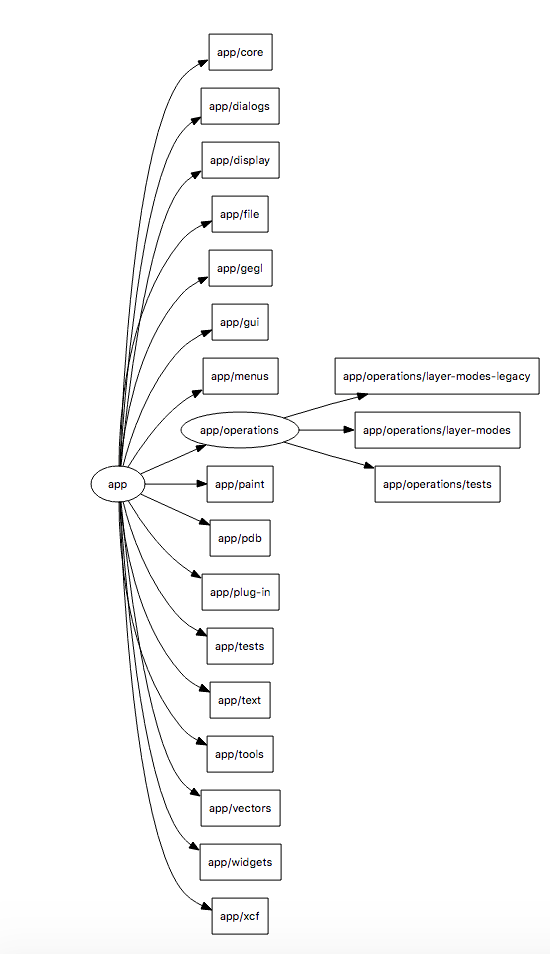
\includegraphics[width=11cm,height=100cm,keepaspectratio]{appfolder.png}
\caption{\label{fig:appfolder}Directory Structure for app folder}
\end{figure}
\section{Entry Point}
While trying to build the application, we looked at MakeFile.am. The following line in MakeFile.am which gave us an idea about the entry point into the program. 
\newline 
\textbf{gimp\_@GIMP\_APP\_VERSION@\_SOURCES = \$(libapp\_sources) main.c}
\newline
Understand C++ has an option to generate a callby graph. Running this on main.c, instantly we can guess that main is not called by anything which further reinforces the idea that main is the entry point into the program. The call by graph for main.c is shown in figure \ref{fig:callbymain}
\begin{figure}
\centering
\includegraphics[width=3cm,height=100cm,keepaspectratio]{callbymain.png}
\caption{\label{fig:callbymain}Callby graph for main.c}
\end{figure}

So looking into the main.c to further reinforce our idea.
 
The main.c has a main function which points to functions that talk about the installation directory.
We did gain a lot of information from the Understand C++ software.
 
Failures: We tried to use Doxygen to generate call graphs for comparison and better understanding. However, the tool crashed on the first go. And on the second go generated quite a bunch of call graphs when run directly on the app directory so will leave this tool aside for now.


\section{Build Process}
Analysis of any application can not be completed without building it. Like every application provide documentation related to how one can build the application on any platform eg Linux, Mac etc. Building any application not only help to compile any application to create executable but end up to helping to figure out what are the entry point with in the code of application.  Like in case of Gimp they have "MakeFile.am" which is a autogenerator file with in "master/app" directory to create "Makefile.in" . If you analyze Makefile.am you will get that "main.c" is the file from were compilation starts.

We tried to use Doxygen to generate call graphs for comparison and better understanding. However, the tool crashed on the first go. And on the second go generated quite a bunch of call graphs when run directly on the master/app directory so will leave this tool aside for now.

Talking about Dependencies required for the Gimp to get build you can check with in GIMP master folder you will find the INSTAL.in file which will tell how to build the application on particular platform with dependencies required. We are using Linux environment to build the application.

To build this process we have two different type of	build system provided one through a Tarball and other  building from latest source (Git).We used the latter one to build the application.

Being a product of GNOME ,gimp use many of their pre existing libraries which they utilize for their other products  as well like GLib , GObject ,GTK+, Cairo, Pango. 

The two major libraries which gimp uses are GEGL and babl which one need to install before building this application. And both can be installed either using tarball or git on system before building. Links for both the libraries are present on wiki page of the application.\cite{wiki}.

Once this is done we are require to just run autogen.sh which is a auto maker for configuration file. Once configuration file is generated we can run it to auto generate makefile. Also this is where you get to know if you have installed all libraries or not. This is the place where we got stuck as I already had a previous gimp installation and did not change the path for the new installation and end up having conflict between both of the installation which got resolved by just changing the default path. Once make file is generated you can run the “make” command  and then “make install”  to complete the build process.

So if we see the major flow of the build after installing all libraries is as follows:
\newline
\textbf{ autogen.sh---config---make---make install}
\newline
\newline
Gimp can be build for three different platform Linux , Mac and Windows. Apart from few problem which I mentioned in the earlier section we also faced following issues.
\begin{itemize}
\item \textbf {We got error for relative path in the prefix.}
If you google you get lot of solution for this and we figured out that the path we are using is not the absolute one so we were able to fix this issue after searching for two three time.
\item \textbf{ Also we got old GTK+ version error. }
As I already had one installation of gimp on my machine 
so when for the first time I ran configuration file it gave me an      
GTK+ old version error which I was able to fix by just making 
An update for the library.
	
\end{itemize}
To Summaries the build process we need to have to install all libraries which are mentioned in the wiki page


\section{Control Flow}
\section{Dependencies}
Gimp has a dependency on many libraries some important ones are as follows:
\begin{enumerate}
\item \textbf{GLib:} \newline
A common library which is basically used in most of the gnome applications, it contains the various utilities and data structures needed by the program in c.
\item \textbf{GEGL:} \newline
It is a graph based image processing library which is used by GIMP in order to support high bit depth images.
\item \textbf{babl:} \newline
It is a support library for GEGL. It is helpful in color-space conversions.
\item \textbf{PDBTypes.h:} \newline
It is helpful in defining enums for various fields contained in PDB.
\item \textbf{GDK:} \newline
It helps by acting as a wrapper around low level functions.
\item \textbf{GObject:} \newline
It is a library which is used to implement C objects.
\end{enumerate}

\section{Algorithms}
To find the underlying algorithms behind the operations performed on GIMP, the wiki for the same had a link to the algorithms used. We expected to find all the underlying algorithms here but encountered a problem. There was only one operation described here shown in figure \ref{fig:algorithm}.

\begin{figure}
\centering
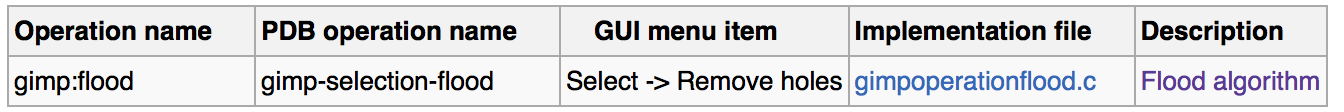
\includegraphics[width=1\textwidth]{algorithm.png}
\caption{\label{fig:algorithm}Documentation on operation algorithms}
\end{figure}

Since this is implemented in the gimpoperationflood.c, the best way to find the algorithms for the other operations performed would be to have a look at where this file is located.
 
The app/operations folder is where this file located. Looking at the other files in the folder, we got an idea of where to look incase we had to change or add any further operations. Since these operations are triggered using the GUI, changing something here would cause us to look at the UI elements to be updated as well.

\section{Problem and Solution}
We already discussed few problem which we faced during previous section here again we are going to put few specific issues which we faced.
\newline
\textbf{Make command stops with the error 'No rule to make target all':} So looking at different solution on line we figured out that with in the configure.ac we missed to update our directory path because of which this error occurred. We can also provide prefix when running the autogen.sh file.
\newline
\textbf{aclocal: error: non-option arguments are not accepted:} Tried editing the project environments setting to check if  ACLOCAL\_FLAGS variable doesn't appear here or is not printed boldly. Also remove if any quotes are present from the  ACLOCAL\_FLAGS

\section{Conclusion}
After doing the analysis of the GIMP code base things which we learned are that if the code is well written with proper documentation its not tough to do the comprehension. In case of Gimp like we already stated in abstract that it has well written code base with proper documentation which give you easy understanding of the code. And when you use different visualization tool it becomes more easy to get proper call graphs which help to locate entry point in code when you build your code. Other thing what we concluded is that, one should not start doing analysis without building the application, building application first ends up letting you know not only entry point in the code but also what all different libraries are required to build the application which in turn sometime are meaning full enough to determine the purpose of application.

\newpage
\begin{thebibliography}{9}
	\bibitem{LocMetrics}
	http://www.locmetrics.com/
	
	\bibitem{cloc} 
	https://github.com/AlDanial/cloc
	
	\bibitem{wiki}
	https://wiki.gimp.org/
	
	
	
\end{thebibliography}
\end{document}